\chapter{Interpolation, Discount Factors and Forward Rates}
\label{interpolation---practical-lesson-3}

In this Chapter we will start to see applications of \texttt{python} to financial calculations.
In particular discount curves and forward rates will be involved, implementing the first utilities that go into a financial module that will be developed throughout this course.
In doing so we will review a widely used mathematical tool: \emph{interpolation}.

\section{Linear Interpolation}
\label{linear-interpolation}

Consider to have few data points, obtained by sampling or experimenting. These points represent the values of a not well known function \(f(x)\), where \(x\) is an independent variable (e.g.~in recording a trip: distances at certain times, \(d = f(t)\)).

It may be necessary to estimate values of the function $f$ at values for which we don't have samples. Interpolation is a method of "constructing" new points within the range of the known data.

Let's clarify the technique with an example.
Assume you are going on holidays by car and that luckily there isn't much traffic so that you can drive at constant speed (which gives a linear relation between traveled space and time i.e.~\(s = v \cdot t\), which means that if you plot the distances \(s\) as a function of the time \(t\) you get a line with slope \(v\)), see Fig.~\ref{fig:samples_for_interpolation}.

\begin{figure}
  \centering
  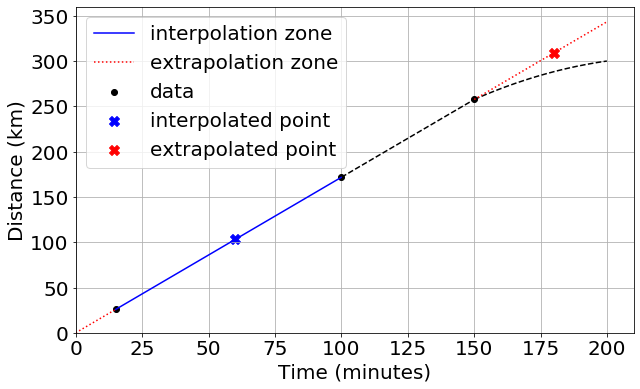
\includegraphics[width=0.7\textwidth]{figures/interp_example1.png}
  \caption{An example of sampling of traveled distances at some time. The red point shows an additional sample taken after the trip velocity has been reduced.}
  \label{fig:samples_for_interpolation}
\end{figure}

Given two samples of the car traveled distance \(s_1\) and \(s_2\) taken at two different times \(t_1\) and \(t_2\) you can linearly interpolate to find your position at different times using the following relations:

\begin{equation}
s = (1 - w)\cdot s_1 + w \cdot s_2
\end{equation}
where $t$ is a generic time at which we want to know the distance $s$ and \(w = \cfrac{t - t_1}{t_2 - t_1}\).

\begin{attention}
\subsubsection{Derivation}
The equation of a line for two points \((t_1, s_1)\) and \((t_2, s_2)\) can be written as:

\begin{equation}
\frac{t - t_1}{t_2 - t_1} = \frac{s - s_1}{s_2 - s_1}
\end{equation}

Setting \(w = \cfrac{t - t_1}{t_2 - t_1}\) and solving for \(s\) we find the desired solution:

\begin{equation}
(s_2 - s_1)\cdot w = s - s_1\quad\implies\quad s = (1 - w)\cdot s_1 + w \cdot s_2
\end{equation}

This formula can also be understood as a weighted average where the weights are inversely related to the distance from the end points to the unknown point ($w_1 = (1 - w) = \cfrac{t_2 - t}{t_2 -t_1}, w_2 = w$), which means that the closer point has more influence than the farther point.
\end{attention}

Back to our example, if
\(s_1 = 25.75~\mathrm{km}\;(@t_1 = 15~\mathrm{min})\) and
\(s_2 = 171.7~\mathrm{km}\;(@t_2 = 100~\mathrm{min})\) let's find distance traveled in 1 hour (interpolation):

\begin{ipython}
s_1 = 25.75 # distance in km
t_1 = 15 	# elapsed time in minutes
s_2 = 171.7
t_2 = 100

t = 60
w = (t - t_1)/(t_2 - t_1)
s = (1 - w)*s_1 + w*s_2
print ("{:.1f} km".format(s))
\end{ipython}
\begin{ioutput}
103.0 km
\end{ioutput}

Always interpret critically your results to guess if they make sense or not and to avoid mistakes. In the previous example we certainly expected something between 25.75 and 171.7~km (our range ends) furthermore since we are looking for the distance at a time which is almost halfway the interval, the result will be somehow in the middle or around 98.6~km. This is indeed more or less what we have got.
This simple kind of reasoning should be applied every time you have a result to quickly judge it.

\begin{curiosity}
\subsubsection{Epic Failure}
The Mars Climate Orbiter \emph{was} a 638~kg (1,407~lb), 326.7~M\$ space probe launched by NASA on December 11, 1998 to study the Martian climate, atmosphere, and surface changes. 

On September 15, 1999, the necessary corrections to speed and direction of the probe were computed in order to place the spacecraft at an optimal position for an orbital insertion maneuver that would bring it around Mars at the proper altitude. 
But one week later communication with the spacecraft was permanently lost as it went into Martian orbital insertion. 

A committee of experts was created to investigate the reasons of 
such failure and they found out that the spacecraft encountered Mars at a lower than foreseen altitude causing either its destruction by atmospheric friction or making it bouncing against the atmosphere re-entering heliocentric orbit after leaving Mars.

The primary cause of this discrepancy was found in one piece of software (supplied by Lockheed Martin) that produced results in "Imperial" units,  while a second system (supplied by NASA) expected those results to be in SI units. Specifically, the software calculated the total impulse produced by thruster in \emph{pound-force seconds}. The trajectory calculation software then used these results, expected to be in \emph{newton seconds}, thus incorrect by a factor of 4.45, to update the predicted position of the spacecraft.
	
NASA took the entire responsibility for having vaporized about 300~M\$ in the Martian atmosphere, mainly for failing to make the appropriate checks and tests that would have caught this unit discrepancy~\cite{bib:mars}.	
\end{curiosity}

\subsubsection{Extrapolation}

If we believe the relation between our variable stays the same ($f(t)$ still linear), we can use the same formula to \emph{extrapolate} values \emph{outside} our initial sample. For example if we keep the same constant velocity in our trip we could check the distance traveled after 3 hours:

\begin{ipython}
t = 180
w = (t - t_1)/(t_2 - t_1)
s = (1 - w)*s_1 + w*s_2
print ("{:.1f} km".format(s))
\end{ipython}
\begin{ioutput}
309.1 km
\end{ioutput}

\subsection{Log-linear Interpolation}
\label{log-linear-interpolation}
When the function $f$ that we want to interpolate is an exponential we can fall back to the previous case by a simple variable transformation. 
Assume the following is the relationship between $p$ and $h$, two generic variables:

\begin{equation}
p = \mathrm{exp}(c \cdot h)
\end{equation}
Applying the logarithm to both sides of the equation gives:

\begin{equation}
s = \mathrm{log}(p) = \mathrm{log}(\mathrm{exp}(c \cdot h)) = c \cdot h
\end{equation}
so there is linear relation between the new variable $s$ and $h$. At this point we can use the results of the previous Section to interpolate for values of $s$, just remember to exponentiate the final result to get the correct $p$. In formulas:

\begin{align}
\label{eq:log_interp}
\begin{gathered}
w = \frac{h - h_1}{h_2 - h_1} \\
s = (1 - w)\cdot s_1 + w \cdot s_2\qquad (\textrm{now } s = \textrm{log}(p))\\
p = \textrm{exp}(s)
\end{gathered}
\end{align}

Let's see another example. Atmospheric pressure decreases with the altitude (i.e.~the highest you flight the lower is the pressure) following an exponential law:

\begin{equation}
p = p_0\cdot e^{-\alpha h}
\end{equation}
where
\begin{itemize}
\tightlist
\item
  \(h\) is the altitude
\item
  \(p_0\) is the pressure at sea level
\item
  \(\alpha\) is a constant
\end{itemize}

Taking the logarithm of each side of the equation we get a linear relation which 
can be interpolated as seen before:

\begin{equation}
s = \mathrm{log}(p) = \mathrm{log}(p_0\cdot e^{-\alpha h})\propto - \alpha \cdot h
\end{equation}

Now assume that we have measured
\(p_1 = 90~\mathrm{kPa}\;(h_1 = 1000~\mathrm{m})\) and
\(p_2 = 40~\mathrm{kPa}\;(h_1 = 7000~\mathrm{m})\) what will be the
atmospheric pressure on top of Mont Blanc (\(4812~\mathrm{m}\)) ? and on top of Mount Everest (\(8848~\mathrm{m}\)) ?

\begin{ipython}
# pressure on top of the Mont Blanc (interpolation)
from math import log, exp

# first we take the logarithm of our measurements to use the linear
# relation to interpolate
h_1 = 1000 # height in meters
s_1 = log(90) # logarithm of the pressure at heigth h1
h_2 = 7000 # height in meters
s_2 = log(40) # logarithm of the pressure at heigth h2

h = 4812
w = (h - h_1)/(h_2 - h_1)
s = (1 - w)*s_1 + w*s_2
print ("{:.1f} kPa".format(exp(s)))
\end{ipython}
\begin{ioutput}
53.8 kPa
\end{ioutput}

\begin{ipython}
h = 8848
w = (h - h_1)/(h_2 - h_1)
s = (1 - w)*s_1 + w*s_2

print ("{:.1f} kPa".format(exp(s)))
\end{ipython}
\begin{ioutput}
31.2 kPa
\end{ioutput}

In this case we check our results by plotting the found pressures on top of the $P$ vs $h$ plot shown on Wikipedia, see Fig~\ref{fig:Pvsh}.

\begin{figure}
\centering
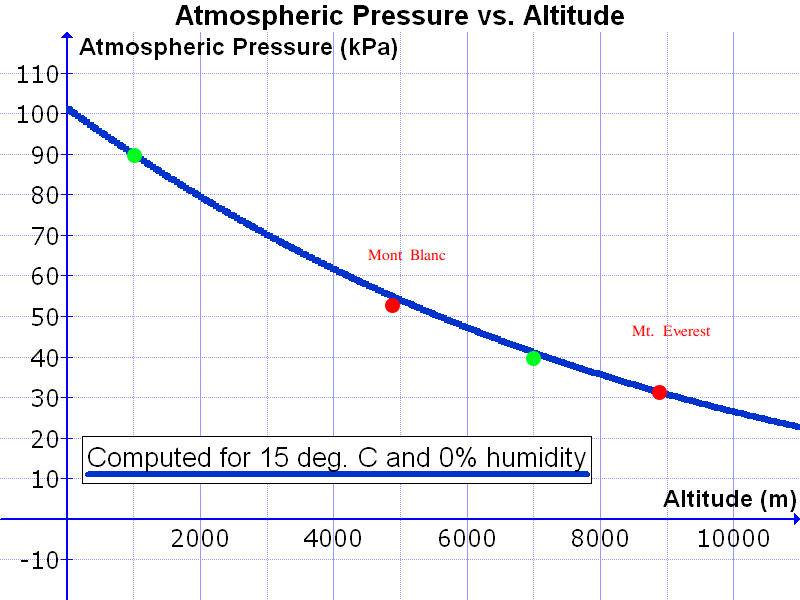
\includegraphics[width=0.7\linewidth]{figures/Atmospheric_Pressure_vs._Altitude.png}
\caption{Atmospheric pressure versus altitude (Wikipedia). Green points
represent our measurements, red points represent
interpolation/extrapolation.}
\label{fig:Pvsh}
\end{figure}

\subsection{Limitations of Interpolation}
Interpolation is just an approximation and works well when either the function $f$ is linear or we are trying to interpolate between two points that are close enough to believe that $f$ is almost linear in that interval.

It can be easily demonstrated that the linear approximation between two points of a given function $f(x)$ gets worse with the second derivative of the function that is approximated ($f''(x)$). This is intuitively correct: the "curvier" the function is, the worse the approximation made with simple linear interpolation becomes, see Fig.~\ref{fig:sine_interp} where we try to interpolate a sine function.

\begin{figure}
  \centering
  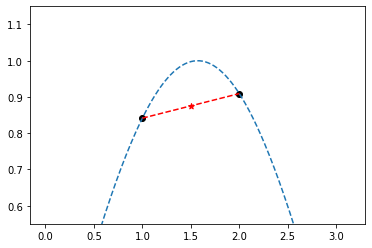
\includegraphics[width=0.7\textwidth]{figures/wrong_interp.png}
  \caption{Trying to approximate a sine function with a line is clearly not going to work unless the interpolation interval is very small.}
  \label{fig:sine_interp}
\end{figure}

To improve the approximation accuracy with complicated curves a polynomial of higher order can be used ($𝑝(𝑥)=𝑎_0 + 𝑎_1 𝑥+ 𝑎_2 𝑥^2+\cdots$), for example in the evaluation of natural logarithm or trigonometric functions. It has to be clear however that going to higher degrees does not always help~\cite{bib:runge}.

\section{Discount Factors}
\label{discount-factors}
The discount factor, $D(T)$, is the factor by which a future cash flow must be multiplied in order to obtain its present value. For a zero-rate (also called spot rate) $r$, and a time to cash flow $T$ (in years), the discount factor is:

\begin{equation}
D(0, T)= \frac {1}{(1+rT)}
\label{eq:discount_factor}
\end{equation}

When the continuously-compounded hypothesis is used the discount factor becomes

\begin{equation}
D(0, T)= e^{-rT}
\label{eq:discount_factor_cc}
\end{equation}

\subsection{Discount Curve Interpolation}
\label{discount-curve-interpolation}

Since discount curves are made of a discrete set of discount factors derived at some dates, we may need to find the factor at some different time; this is a typical financial application of interpolation.

To develop some \texttt{python} code which interpolates a discount curve are needed:

\begin{itemize}
\tightlist
\item a list of pillars dates specifying the value dates of the given discount factors, \(t_0,...,t_{n-1}\);
\item a list of given discount factors, \(D(t_0),...,D(t_{n-1})\);
\item a pricing date (`today') which corresponds to \(t=0\).
\end{itemize}

The input argument to the function will be the value date at which we want to interpolate the discount factor. Since the discount factor can be expressed as an exponential the log-linear interpolation can be used:

\begin{equation}
\begin{gathered}
d(t_i)=\mathrm{ln}(D(t_i))\\
d(t) = (1-w)d(t_i) + wd(t_{i+1});\quad w=\frac{t-t_i}{t_{i+1}-t_i}\\
D(t) = \mathrm{exp}(d(t))
\end{gathered}
\end{equation}
where \(i\) is such that \(t_i \le t \le t_{i+1}\)

Instead of reinventing the wheel and performing the interpolation with homemade code, 
the function \texttt{interp}, provided by the module \texttt{numpy}, is used. 
Say we want to interpolate the points at $x = 2.5$ given the following values:

\begin{ipython}
import numpy as np

xp = [0, 1, 5]
fp = [0, 2, 4]
np.interp(2.5, xp, fp)
\end{ipython}
\begin{ioutput}
2.75
\end{ioutput}

Since discount factors are an essential part for every financial calculation and we will keep using them everywhere, a \texttt{python} class which manages discount factors and curves is develop, using an object oriented approach.
This class, that we name \texttt{DiscountCurve}, should have as attributes the pillar dates with the corresponding discount factors and at least a method to interpolate discount factors.

When dealing with discount factors we need to be careful though. \texttt{numpy.interp} only accepts numbers or a list of numbers as argument i.e. it doesn't automatically convert or interpret dates as numbers and doesn't know how to interpolate them. So we need to do the conversion ourselves before passing any date to the interpolation function. This transformation will be implemented directly in the constructor of the class by replacing each date with the number of days from a reference date ($t_0$).

Furthermore we also attempted a simple optimization of the code, in the constructor we are going to compute also the logarithm of the input discount factors, so that we can save some computation time with respect to doing the log at every call of the interpolation method. 

\begin{ipython}
import math
import numpy
from datetime import date

class DiscountCurve:
    def __init__(self, today, pillar_dates, discount_factors):
        self.today = today
        self.pillar_dates = pillar_dates
        self.discount_factors = discount_factors
        self.log_dfs = [math.log(discount_factor) \
            for discount_factor in self.discount_factors]
        self.pillar_days = [(pillar_date - self.today).days \
            for pillar_date in self.pillar_dates]

    def df(self, d):
        d_days = (d - self.today).days
        interp_log_df = \
            numpy.interp(d_days, self.pillar_days, self.log_dfs)
        return math.exp(interp_log_df)
\end{ipython}

\begin{finmarkets}
This class is going to be the first step in the creation of a \texttt{python} financial library,
so copy the code into a separate file called \texttt{finmarkets.py} so that you can later reuse 
it.
Also be sure that the code is well documented in its part.	
\end{finmarkets}

Assume we have three discount factors, we can now use our new class to create the corresponding
discount curve. Then the \texttt{df} method provides discount factors on every date within the interval of the given pillar dates.

\begin{ipython}
from datetime import date
from finmarkets import DiscountCurve

today_date = date(2019, 10, 1)
pillar_dates = [date(2019, 10, 1), date(2020, 10, 1), date(2021, 10, 1)]
discount_factors = [1.0, 0.97, 0.72]
curve = DiscountCurve(today_date, pillar_dates, discount_factors)
d0 = date(2020, 1, 1)
df0 = curve.df(d0, today_date, pillar_dates, discount_factors)
print (df0)
\end{ipython}
\begin{ioutput}
0.9923728228571693
\end{ioutput}
\begin{ipython}
d1 = date(2021, 1, 1)
df1 = curve.df(d1, today_date, pillar_dates, discount_factors)
print (df1)
\end{ipython}
\begin{ioutput}
0.8997999273630835
\end{ioutput}

A very useful way to check the correctness of a result is by plotting it. So let's see what this looks like when plotted on a semi-log graph and if it makes sense, Fig.~\ref{fig:log_discount_curve}.

\begin{ipython}
from matplotlib import pyplot as plt
import matplotlib.dates as mdates
plt.plot(pillar_dates, discount_factors, marker='o')
plt.plot(d0, df0, marker='X')
plt.plot(d1, df1, marker='X')
plt.gca().xaxis.set_major_formatter(mdates.DateFormatter('%m/%d/%Y'))
plt.gca().xaxis.set_major_locator(mdates.YearLocator())
plt.grid(True)
plt.yscale("log")
plt.show()
\end{ipython}

\begin{figure}[htb]
	\centering
	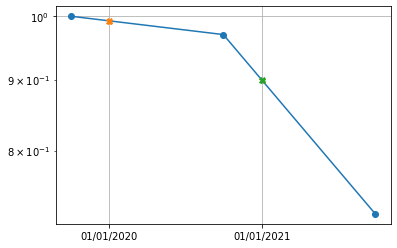
\includegraphics[width=0.7\textwidth]{figures/log_discount_curve}
	\caption{Plot of the discount curve defined in the text and of the two computed
		discount factors with semi-log scale.}
	\label{fig:log_discount_curve}
\end{figure}
\noindent
Let's see what it looks like when plotted on a linear graph too, Fig.~\ref{fig:linear_discount_curve}.
\begin{ipython}
plt.plot(pillar_dates, discount_factors, marker='o')
plt.plot(d0, df0, marker='X')
plt.plot(d1, df1, marker='X')
plt.gca().xaxis.set_major_formatter(mdates.DateFormatter('%m/%d/%Y'))
plt.gca().xaxis.set_major_locator(mdates.YearLocator())
plt.grid(True)
plt.show()
\end{ipython}

\begin{figure}[htb]
	\centering
	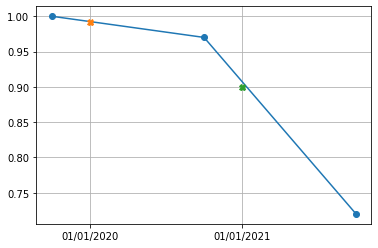
\includegraphics[width=0.7\textwidth]{figures/linear_discount_curve}
	\caption{Plot of the discount curve defined in the text and of the two computed
		discount factors with linear scale.}
	\label{fig:linear_discount_curve}
\end{figure}
\noindent
Discrepancies in the linear plot are most likely due to rounding.

\section{Forward Rates}\label{calculating-forward-rates}
A forward rate is an interest rate applicable to a financial transaction that will take place in the future. It can be considered as the market's expectations for future prices and can serve as an indicator of how it believes will perform.

Contrary the \emph{spot rate} is used by buyers and sellers looking to make an immediate purchase or sale, and it cannot be an indicator of market expectations.

Forward rates are calculated from the spot rate by exploiting the no arbitrage condition which states that investing at rate \(r_1\) for the period \((0, T_1)\) and then \emph{re-investing} at rate \(r_{1,2}\) for the time period \((T_1, T_2)\) is equivalent to invest at rate \(r_2\) for the full time period \((0, T_2)\). Essentially two investors shouldn't be able to earn money from arbitraging between different interest periods. That said:

\begin{equation}
(1+r_1 T_1)(1+r_{1,2}(T_2 - T_1)) = 1 + r_2 T_2
\label{eq:no_arbitrage_r}
\end{equation}
Solving for \(r_{1,2}\) leads to

\begin{equation}
F(T_1, T_2) = r_{1,2} = \frac{1}{T_2 - T_1}\Big(\frac{1+r_2 T_2}{1+r_1 T_1} - 1 \Big)
\label{eq:forward_rate_simple}
\end{equation}
\vspace{1cm}
The same expression in terms of the discount factor of Eq.\ref{eq:discount_factor} becomes
\begin{equation}
F(T_1, T_2) = \frac{1}{T_2 - T_1}\Big(\frac{D(0, T_1)}{D(0, T_2)} - 1 \Big)
\end{equation}
Considering continuously compounded rates instead Eq.~\ref{eq:no_arbitrage_r} can be written as
\begin{equation*}
e^{{(r}_{2}T_{2})}=e^{{(r}_{1}T_{1})}\ast \ e^{\left(r_{1,2} \left(T_{2}-T_{1}\right)\right)}
\end{equation*}
and the corresponding expression for the forward rate is
\begin{equation}
F(T_1, T_2) = r_{1,2} = \frac {1}{T_{2}-T_{1}}(\ln D(0,T_{1})-\ln D(0,T_{2}))
\quad(\textrm{since now } D(0, T_i)=e^{-r_i T_i})
\label{eq:forward_rate_continous}
\end{equation}

We now write a very simple \texttt{ForwardRateCurve} class which doesn't compute discount factors or other fancy values but it is just a container for a list of forward rates and can interpolates between them.
Also this class goes into the \texttt{finmarkets} module and will be used to define the LIBOR curve needed throughout future Chapters.

In this case it is enough to write a class that has three attributes: a set of pillar dates and the corresponding forward rates. The reference date to convert the pillars for the interpolation (i.e. today) is taken from the first item of the pillar list. There will be just a single method \texttt{forward\_rate} to return an interpolated rate.

\begin{ipython}
import numpy

class ForwardRateCurve(object):
    def __init__(self, pillar_dates, rates):
        self.today = pillar_dates[0]
        self.rates = rates
        self.pillar_days = [(pillar_date - self.today).days \
        for pillar_date in pillar_dates]

    def forward_rate(self, d):
        d_days = (d - self.today).days
        return numpy.interp(d_days, self.pillar_days, self.rates)
\end{ipython}

\section{Multi-curve Framework}
\label{sec:financial-crisis}

Prior to the 2008 financial crisis, interbank deposits posed little 
credit/liquidity issues, interbank lending rates (IBOR rates, e.g. LIBOR, EURIBOR)
were essentially a good proxy for risk free rates. 
Basis swap spreads were negligible and thereby neglected. 

Looking at the historical series of the EURIBOR (6M) rate versus the EONIA 
Overnight Indexed Swap (OIS-6M) rate over the time interval 2006-2011 in Fig.~\ref{fig:credit_crunch} it becomes
apparent how before August 2007 the two rates display strictly overlapping trends differing of no more than 6 bps.

\begin{figure}[htb]
	\centering
	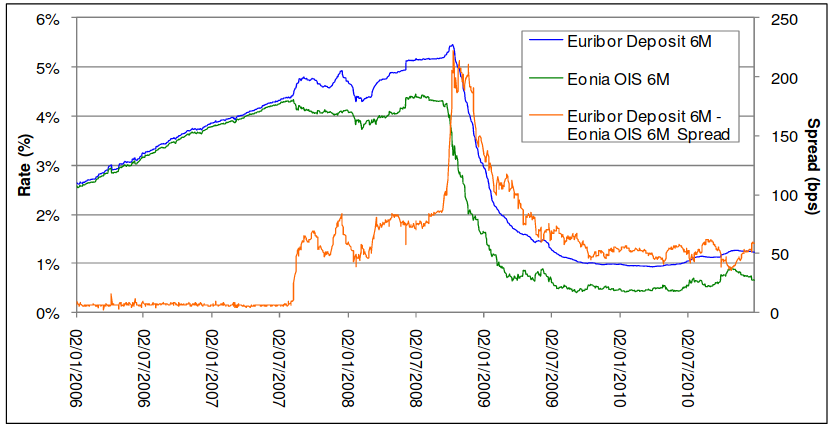
\includegraphics[width=0.9\linewidth]{figures/credit_crunch.png}
	\caption{Historical series of EURIBOR 6M rate versus EONIA OIS 6M rate. The corresponding spread 
		is shown on the right axis (Jan. 06 - Dec. 10 window, source: Bloomberg).}
	\label{fig:credit_crunch}
\end{figure}

A single yield curve constructed out of selected deposit rates, FRA/EDF rates and swap rates served both the cash flow projection and discounting purposes.

During the 2008 financial crisis, the failure of some banks however proved that interbank lending rates (e.g. LIBOR, EURIBOR\ldots) were not risk-free. Meanwhile there was also significant counterparty credit risk arising from derivative transactions that were not subject to collateral or margin calls. Basis swap spreads greatly widened, and persist to this day. 

Still looking at Fig.~\ref{fig:credit_crunch} it is clear how in August 2007 a sudden increase of the EURIBOR rate and a simultaneous decrease of the OIS rate leads to the explosion of the corresponding basis spread, touching the peak of 222 bps in October 2008, when Lehman Brothers filed for bankruptcy. Successively the basis has sensibly reduced and stabilized between 40 bps and 60 bps (notice that the precrisis level has never been recovered). 
The same effect is observed for other similar couples of series, e.g. EURIBOR 3M vs OIS 3M.

The existence of such significant basis swap spreads reflects the fact that after the crisis the interest rate market has been segmented into subareas corresponding to instruments with different underlying rate tenors, characterized by different rate dynamics. 

Traditional single curve based pricing approach ignores these differences. It mixes different underlying rate tenors and incorporates different rate dynamics, eventually leads to inconsistency.
After the crisis, the market practice has thus evolved to take into account the new market information (e.g. the basis swap spreads, collateralization, etc.), that translate into the additional requirement of homogeneity and funding. The homogeneity requirement means that interest rate derivatives with a given underlying rate tenor must be priced and hedged using vanilla interest rate market instruments with the same underlying. The funding requirement means that 
the discount rate of any cash flow generated by the derivative must be consistent, by no-arbitrage, with the funding rate associated with that cash flow. 

Driven by the crisis, many derivative contracts have been updated to include permissible credit mitigants for a transaction, such as netting and collateralization in cash.
Since standard agreements stipulate daily margination on collateral and the cash collateral earns a return at overnight rate, overnight rate becomes a natural choice for the risk-free discount rate or the funding rate. This is referred to as \emph{OIS discounting}.

The large spread between risk free rate and interbank lending rate during and after 2008 financial crisis it is not possible anymore to use a single curve for discounting and derivative valuation. The traditional single curve used for both  cash flow projection and discounting turned out to be obsolete. The markets have since nearly switched to multi-curve framework. 

For example, if we want to calculate the net present value (NPV) of a forward 6-month LIBOR coupon, we need to simultaneously use two different discount curves: 

\begin{itemize}
\tightlist
\item the 6-month LIBOR curve for determining the forward rate;
\item the EONIA curve for discounting the expected cash flow.
\end{itemize}

%The reason of the abrupt divergence between the Euribor and OIS rates can be explained by considering both the monetary policy decisions adopted by international authorities in response to the financial turmoil, and the impact of the credit crunch on both credit and liquidity risk perception of the market, coupled with the different financial meaning and dynamics of these rates.

%\begin{itemize}
%\tightlist
%\item
%  The Euribor rate is the reference rate for over-the-counter (OTC)
%  transactions in the Euro area. It is defined as the rate at which
%  Euro inter-bank deposits are being offered within the EMU zone by one
%  prime bank to another at 11:00 a.m. Brussels time. The rate fixings
%  for a strip of 15 maturities (from one day to one year) are
%  constructed as the average of the rates submitted (excluding the
%  highest and lowest 15\% tails) by a panel of 42 banks, selected
%  among the EU banks with the highest volume of business in the Euro
%  zone money markets, plus some large international bank from non-EU
%  countries with important euro zone operations. \emph{Thus, Euribor
%  rates reflect the average cost of funding of banks in the inter bank
%  market at each given maturity. During the crisis the solvency and
%  solidity of the whole financial sector was brought into question and
%  the credit and liquidity risk and uremia associated to inter-bank
%  counter-parties sharply increased.} The Euribor rates immediately
%  reflected these dynamics and raise to their highest values over more
%  than 10 years. As seen in the plot above, the Euribor 6M rate suddenly
%  increased on August 2007 and reached 5.49\% on 10th October 2008.
%\item
%  The EONIA rate is the reference rate for overnight OTC transactions in
%  the Euro area. It is constructed as the average rate of the overnight
%  transactions (one day maturity deposits) executed during a given
%  business day by a panel of banks on the inter-bank money market,
%  weighted with the corresponding transaction volumes. \emph{The EONIA
%  Contribution Panel coincides with the Euribor Contribution Panel, thus
%  EONIA rate includes information on the short term (overnight)
%  liquidity expectations of banks in the Euro money market. It is also
%  used by the European Central Bank (ECB) as a method of effecting and
%  observing the transmission of its monetary policy actions. During the
%  crisis the central banks were mainly concerned about stabilizing the
%  level of liquidity in the market, thus they reduced the level of the
%  official rates.} Furthermore, the daily tenor of the EONIA rate makes
%  negligible the credit and liquidity risks reflected on it: for this
%  reason the OIS rates are considered the best proxies available in the
%  market for the risk-free rate.
%\end{itemize}

Our financial library has to implement the following calculation

\[\mathrm{NPV} = D_{\mathrm{EONIA}}(T_1) \cdot \frac{1}{T_2-T_1}\Big(\frac{D_{\mathrm{LIBOR}}(T_1)}{D_{\mathrm{LIBOR}}(T_2)} - 1 \Big)\]
\noindent
In order to do so we can extend the \texttt{DiscountCurve} class with a \texttt{forward\_rate}
method

\begin{ipython}
class DiscountCurve:
    ...
    def forward_rate(self, d1, d2):
        return (self.df(d1) / self.df(d2) - 1.0) * \
            (365.0 / ((d2 - d1).days))
\end{ipython}

As an example let's define EONIA and LIBOR curves and compute the net present value of the forward 6-month LIBOR coupon mentioned before.

\begin{ipython}
from finmarkets import DiscountCurve

today_date = date (2020, 1, 1)
t1 = date(2020, 4, 1)
t2 = date(2020, 10, 1)
pillar_dates_eonia = [date(2020, 1, 1), date(2021, 1, 1), date(2022, 10 ,1)]
df_eonia = [1.0, 0.97, 0.72]
pillar_dates_libor = [date(2020, 1, 1), date(2020, 6, 1), date(2020, 12 ,1)]
df_libor = [1.0, 0.95, 0.90]
eonia_curve = DiscountCurve(today_date, pillar_dates_eonia, df_eonia)
libor_curve = DiscountCurve(today_date, pillar_dates_libor, df_libor)
npv = eonia_curve.df(t1) * libor_curve.forward_rate(t1, t2)
npv_pre2008 = libor_curve.df(t1) * libor_curve.forward_rate(t1, t2)

print ("NPV post 2008:", npv)
print ("NPV pre 2008:", npv_pre2008)
\end{ipython}
\begin{ioutput}
NPV post 2008: 0.11533243116069992
NPV pre 2008: 0.11269481011359303
\end{ioutput}

\subsection{Transitioning away from LIBOR~\cite{bib:str}}
A working group on euro risk-free rates was established to identify and recommend risk-free rates that could serve as a basis for an alternative to current benchmarks used in a variety of financial
instruments and contracts in the euro area, such as the euro overnight index average (EONIA) and the euro interbank offered rate (EURIBOR). 

The group recommended on September 2018 that the euro short-term rate (STR) be used as the risk-free rate for the euro area and is now focused on supporting the market with transitioning.
The ECB published the STR for the first time on 2nd October 2019, reflecting trading activity on 1st October 2019.

The working group recommends that market participants should gradually replace EONIA with the STR as a reference rate for all products and contracts and make all necessary adjustments for using the STR as their standard benchmark The working group recommends the STR plus a fixed spread of 8.5
basis points as the EONIA fallback rate for all products and purposes. The working group recommends that market participants should: consider, whenever feasible and appropriate, no longer entering into new contracts referencing EONIA, in particular new contracts maturing after 31 December 2021, as EONIA will cease to exist after that date.

%The working group is also looking at identifying fallbacks for
%EURIBOR based on the STR. Both backward and forward-looking
%options are being considered. As part of its work on forward-looking
%options, in March 2019 the working group recommended a
%methodology based on (tradable) overnight index swap (OIS) quotes
%for calculating a STR-based forward-looking term structure and later
%invited benchmark administrators to express their interest in
%producing such a term structure.

\section{Exercises}
\begin{question}
Python has a useful command called \texttt{assert} which can be used for checking that a given condition is satisfied, and raising an error if the condition is not satisfied.

The following line does not cause an error, in fact it does nothing since 1 is lower than 2, hence the condition is met.

\lstinline[language=iPython]|assert 1 < 2|

\noindent
This causes an error (the condition is evaluated to false). 

\lstinline[language=iPython]|assert 1 > 2|

\noindent
\texttt{assert} can take a second argument with a message to display in case of failure.

\lstinline[language=iPython]|assert 1 > 2, "Two is greater than one"|

\noindent
Now takes the \texttt{df} function from the Chapter on Discounting and modify it by adding some assertions to check that:

\begin{itemize}
\item the pillar date list contains at least 2 elements;
\item the pillar date list has the same length as the discount factor one;
\item the first pillar date is equal to the today's date;
\item the value date (first argument \texttt{d}) is greater or equal to the first pillar date and also less than or equal to the last pillar date.
\end{itemize}

Then try using the function with some invalid data to make sure that your assertions are correctly checking the desired conditions
\end{question}

\begin{solution}
\end{solution}

\begin{ipython}
# import modules and objects that we need
from datetime import date
import numpy
import math

today_date = date(2017, 10, 1)
pillar_dates = [date(2017, 10, 1),
date(2018, 10, 1),
date(2019, 10, 1)]
discount_factors = [1.0, 0.95, 0.8]

def df(d, observation_date, pillar_dates, discount_factors):
    ############## CHECKS ################
    assert len(pillar_dates) >= 2, " need at least 2 pillar dates"
    assert len(pillar_dates) == len(discount_factors), \
        "number of pillar dates should be equal to \
         the number of pillar discount factors"
    assert observation_date == pillar_dates[0], \
        "first pillar date should be the observation date"
    assert pillar_dates[0] <= d <= pillar_dates[-1], \
        "Invalid value date %s" % (d)
    ############## END OF CHECKS ################
    log_discount_factors = []
    for discount_factor in discount_factors:
        log_discount_factors.append(math.log(discount_factor))
    pillar_days = []
    for pillar_date in pillar_dates:
        pillar_days.append((pillar_date - observation_date).days)
    d_days = (d - observation_date).days
    interpolated_log_discount_factor = \
        numpy.interp(d_days, pillar_days, log_discount_factors)
    return math.exp(interpolated_log_discount_factor)

df(date(2019, 1, 1), today_date, pillar_dates, discount_factors)

0.9097285910181567
\end{ipython}

%\begin{question}
%Copy into the file \texttt{finmarkets.py} the function used to compute Black Scholes formula used in Ex.~\ref{ex:BS2}. This is another utility for our financial library. Then repeat Ex.~\ref{ex:BS2} now using the version of the Black and Scholes formula in the \texttt{finmarkets} module.
%\end{question}
%
%\begin{solution}
%\begin{tcolorbox}[size=fbox, boxrule=1pt, colback=cellbackground, colframe=cellborder]
%\begin{Verbatim}[commandchars=\\\{\}]
%\PY{k}{import} \PY{n}{finmarkets}
%        
%\PY{n}{s} \PY{o}{=} \PY{l+m+mi}{800}
%\PY{c+c1}{\PYZsh{} strikes expressed as \PYZpc{} of spot price}
%\PY{n}{moneyness} \PY{o}{=} \PY{p}{[} \PY{l+m+mf}{0.5}\PY{p}{,} \PY{l+m+mf}{0.75}\PY{p}{,} \PY{l+m+mf}{0.825}\PY{p}{,} \PYZbs{}
%             \PY{l+m+mf}{1.0}\PY{p}{,} \PY{l+m+mf}{1.125}\PY{p}{,} \PY{l+m+mf}{1.25}\PY{p}{,} \PY{l+m+mf}{1.5} \PY{p}{]}
%\PY{n}{vol} \PY{o}{=} \PY{l+m+mf}{0.3}
%\PY{n}{ttm} \PY{o}{=} \PY{l+m+mf}{0.75}
%\PY{n}{r} \PY{o}{=} \PY{l+m+mf}{0.005}
%
%\PY{n}{result} \PY{o}{=} \PY{p}{\PYZob{}}\PY{p}{\PYZcb{}}
%\PY{k}{for} \PY{n}{m} \PY{o+ow}{in} \PY{n}{moneyness}\PY{p}{:}
%    \PY{n}{result}\PY{p}{[}\PY{n}{s}\PY{o}{*}\PY{n}{m}\PY{p}{]} \PY{o}{=} \PY{n}{finmarkets.call}\PY{p}{(}\PY{n}{s}\PY{p}{,} \PY{n}{m}\PY{o}{*}\PY{n}{s}\PY{p}{,} \PY{n}{r}\PY{p}{,} \PY{n}{vol}\PY{p}{,} \PY{n}{ttm}\PY{p}{)}
%\PY{n}{result}
%
%\{400.0: 401.66074527896365,
%  600.0: 213.9883852521275,
%  660.0: 166.85957363897393,
%  800.0: 84.03697017660357,
%  900.0: 47.61880394696229,
%  1000.0: 25.632722952585738,
%  1200.0: 6.655275227771156\}
%\end{Verbatim}
%\end{tcolorbox}
%\end{solution}

%\begin{question}
%Following the steps outlined in Chapter Discount Factors, implement a \texttt{DiscountCurve} class and add it to \texttt{finmarkets} module. The class should have as attributes the pillar dates and the corresponding discount factors and two methods, one to interpolate discount factors and another to calculate forward rates.
%Finally using that class compute the forward 6M LIBOR coupon using the curves given below in pre and post 2008 crisis way.
%
%\textbf{Input:}
%\begin{Shaded}
%\begin{Highlighting}[]
%\NormalTok{observation_date }\OperatorTok{=}\NormalTok{ date (}\DecValTok{2020}\NormalTok{, }\DecValTok{1}\NormalTok{, }\DecValTok{1}\NormalTok{)}
%\NormalTok{t1 }\OperatorTok{=}\NormalTok{ date(}\DecValTok{2020}\NormalTok{,}\DecValTok{4}\NormalTok{, }\DecValTok{1}\NormalTok{)}
%\NormalTok{t2 }\OperatorTok{=}\NormalTok{ date(}\DecValTok{2020}\NormalTok{, }\DecValTok{10}\NormalTok{, }\DecValTok{1}\NormalTok{)}
%
%\CommentTok{# for EONIA}
%\NormalTok{pillar_dates_eonia }\OperatorTok{=}\NormalTok{ [date(}\DecValTok{2020}\NormalTok{ , }\DecValTok{1}\NormalTok{ ,}\DecValTok{1}\NormalTok{), }
%\NormalTok{                      date(}\DecValTok{2021}\NormalTok{, }\DecValTok{1}\NormalTok{, }\DecValTok{1}\NormalTok{), }
%\NormalTok{                      date(}\DecValTok{2022}\NormalTok{, }\DecValTok{10}\NormalTok{ ,}\DecValTok{1}\NormalTok{)]}
%\NormalTok{discount_factors_eonia }\OperatorTok{=}\NormalTok{ [}\FloatTok{1.0}\NormalTok{, }\FloatTok{0.97}\NormalTok{, }\FloatTok{0.72}\NormalTok{]}
%
%\CommentTok{# for LIBOR 6M}
%\NormalTok{pillar_dates_libor }\OperatorTok{=}\NormalTok{ [date(}\DecValTok{2020}\NormalTok{, }\DecValTok{1}\NormalTok{ ,}\DecValTok{1}\NormalTok{), }
%\NormalTok{                      date(}\DecValTok{2020}\NormalTok{, }\DecValTok{6}\NormalTok{, }\DecValTok{1}\NormalTok{), }
%\NormalTok{                      date(}\DecValTok{2020}\NormalTok{, }\DecValTok{12}\NormalTok{ ,}\DecValTok{1}\NormalTok{)]}
%\NormalTok{discount_factors_libor }\OperatorTok{=}\NormalTok{ [}\FloatTok{1.0}\NormalTok{, }\FloatTok{0.95}\NormalTok{, }\FloatTok{0.90}\NormalTok{]}
%\end{Highlighting}
%\end{Shaded}
%\end{question}
%
%\begin{solution}
%\begin{tcolorbox}[size=fbox, boxrule=1pt, pad at break*=1mm,colback=cellbackground, colframe=cellborder]
%\begin{Verbatim}[commandchars=\\\{\}]
%\PY{k+kn}{import} \PY{n+nn}{math}
%\PY{k+kn}{import} \PY{n+nn}{numpy}
%\PY{k+kn}{from} \PY{n+nn}{datetime} \PY{k}{import} \PY{n}{date}
%
%\PY{k}{class} \PY{n+nc}{DiscountCurve}\PY{p}{:}
%
%    \PY{k}{def} \PY{n+nf}{\PYZus{}\PYZus{}init\PYZus{}\PYZus{}}\PY{p}{(}\PY{n+nb+bp}{self}\PY{p}{,} \PY{n}{today}\PY{p}{,} \PY{n}{pillar\PYZus{}dates}\PY{p}{,} \PY{n}{discount\PYZus{}factors}\PY{p}{)}\PY{p}{:}
%        \PY{n+nb+bp}{self}\PY{o}{.}\PY{n}{today} \PY{o}{=} \PY{n}{today}
%        \PY{n+nb+bp}{self}\PY{o}{.}\PY{n}{pillar\PYZus{}dates} \PY{o}{=} \PY{n}{pillar\PYZus{}dates}
%        \PY{n+nb+bp}{self}\PY{o}{.}\PY{n}{discount\PYZus{}factors} \PY{o}{=} \PY{n}{discount\PYZus{}factors}
%
%    \PY{k}{def} \PY{n+nf}{df}\PY{p}{(}\PY{n+nb+bp}{self}\PY{p}{,} \PY{n}{d}\PY{p}{)}\PY{p}{:}
%        \PY{n}{log\PYZus{}discount\PYZus{}factors} \PY{o}{=} \PYZbs{}
%          \PY{p}{[}\PY{n}{math}\PY{o}{.}\PY{n}{log}\PY{p}{(}\PY{n}{discount\PYZus{}factor}\PY{p}{)} 
%           \PY{k}{for} \PY{n}{discount\PYZus{}factor} \PY{o+ow}{in} \PY{n+nb+bp}{self}\PY{o}{.}\PY{n}{discount\PYZus{}factors}\PY{p}{]}
%        \PY{n}{pillar\PYZus{}days} \PY{o}{=} \PY{p}{[}\PY{p}{(}\PY{n}{pillar\PYZus{}date} \PY{o}{\PYZhy{}} \PY{n+nb+bp}{self}\PY{o}{.}\PY{n}{today}\PY{p}{)}\PY{o}{.}\PY{n}{days} 
%                       \PY{k}{for} \PY{n}{pillar\PYZus{}date} \PY{o+ow}{in} \PY{n+nb+bp}{self}\PY{o}{.}\PY{n}{pillar\PYZus{}dates}\PY{p}{]}
%        \PY{n}{d\PYZus{}days} \PY{o}{=} \PY{p}{(}\PY{n}{d} \PY{o}{\PYZhy{}} \PY{n+nb+bp}{self}\PY{o}{.}\PY{n}{today}\PY{p}{)}\PY{o}{.}\PY{n}{days}
%        \PY{n}{interpolated\PYZus{}log\PYZus{}discount\PYZus{}factor} \PY{o}{=} \PYZbs{}
%            \PY{n}{numpy}\PY{o}{.}\PY{n}{interp}\PY{p}{(}\PY{n}{d\PYZus{}days}\PY{p}{,} \PY{n}{pillar\PYZus{}days}\PY{p}{,} \PY{n}{log\PYZus{}discount\PYZus{}factors}\PY{p}{)}
%        \PY{k}{return} \PY{n}{math}\PY{o}{.}\PY{n}{exp}\PY{p}{(}\PY{n}{interpolated\PYZus{}log\PYZus{}discount\PYZus{}factor}\PY{p}{)}
%
%    \PY{k}{def} \PY{n+nf}{forward\PYZus{}rate}\PY{p}{(}\PY{n+nb+bp}{self}\PY{p}{,} \PY{n}{d1}\PY{p}{,} \PY{n}{d2}\PY{p}{)}\PY{p}{:}
%        \PY{k}{return} \PY{p}{(}\PY{n+nb+bp}{self}\PY{o}{.}\PY{n}{df}\PY{p}{(}\PY{n}{d1}\PY{p}{)} \PY{o}{/} \PY{n+nb+bp}{self}\PY{o}{.}\PY{n}{df}\PY{p}{(}\PY{n}{d2}\PY{p}{)} \PY{o}{\PYZhy{}} \PY{l+m+mf}{1.0}\PY{p}{)} \PY{o}{*} \PYZbs{}
%                \PY{p}{(}\PY{l+m+mf}{365.0} \PY{o}{/} \PY{p}{(}\PY{p}{(}\PY{n}{d2} \PY{o}{\PYZhy{}} \PY{n}{d1}\PY{p}{)}\PY{o}{.}\PY{n}{days}\PY{p}{)}\PY{p}{)}
%\end{Verbatim}
%\end{tcolorbox}
%
%\begin{tcolorbox}[breakable, size=fbox, boxrule=1pt, pad at break*=1mm,colback=cellbackground, colframe=cellborder]
%\begin{Verbatim}[commandchars=\\\{\}]
%\PY{k+kn}{from} \PY{n+nn}{finmarkets} \PY{k}{import} \PY{n}{DiscountCurve}
%
%\PY{n}{observation\PYZus{}date} \PY{o}{=} \PY{n}{date} \PY{p}{(}\PY{l+m+mi}{2020}\PY{p}{,} \PY{l+m+mi}{1}\PY{p}{,} \PY{l+m+mi}{1}\PY{p}{)}
%\PY{n}{t1} \PY{o}{=} \PY{n}{date}\PY{p}{(}\PY{l+m+mi}{2020}\PY{p}{,}\PY{l+m+mi}{4}\PY{p}{,} \PY{l+m+mi}{1}\PY{p}{)}
%\PY{n}{t2} \PY{o}{=} \PY{n}{date}\PY{p}{(}\PY{l+m+mi}{2020}\PY{p}{,} \PY{l+m+mi}{10}\PY{p}{,} \PY{l+m+mi}{1}\PY{p}{)}
%
%\PY{c+c1}{\PYZsh{} for EONIA}
%\PY{n}{pillar\PYZus{}dates\PYZus{}eonia} \PY{o}{=} \PY{p}{[}\PY{n}{date}\PY{p}{(}\PY{l+m+mi}{2020} \PY{p}{,} \PY{l+m+mi}{1} \PY{p}{,}\PY{l+m+mi}{1}\PY{p}{)}\PY{p}{,} 
%                      \PY{n}{date}\PY{p}{(}\PY{l+m+mi}{2021}\PY{p}{,} \PY{l+m+mi}{1}\PY{p}{,} \PY{l+m+mi}{1}\PY{p}{)}\PY{p}{,} 
%                      \PY{n}{date}\PY{p}{(}\PY{l+m+mi}{2022}\PY{p}{,} \PY{l+m+mi}{10} \PY{p}{,}\PY{l+m+mi}{1}\PY{p}{)}\PY{p}{]}
%\PY{n}{discount\PYZus{}factors\PYZus{}eonia} \PY{o}{=} \PY{p}{[}\PY{l+m+mf}{1.0}\PY{p}{,} \PY{l+m+mf}{0.97}\PY{p}{,} \PY{l+m+mf}{0.72}\PY{p}{]}
%
%\PY{c+c1}{\PYZsh{} for LIBOR 6M}
%\PY{n}{pillar\PYZus{}dates\PYZus{}libor} \PY{o}{=} \PY{p}{[}\PY{n}{date}\PY{p}{(}\PY{l+m+mi}{2020}\PY{p}{,} \PY{l+m+mi}{1} \PY{p}{,}\PY{l+m+mi}{1}\PY{p}{)}\PY{p}{,} 
%                      \PY{n}{date}\PY{p}{(}\PY{l+m+mi}{2020}\PY{p}{,} \PY{l+m+mi}{6}\PY{p}{,} \PY{l+m+mi}{1}\PY{p}{)}\PY{p}{,} 
%                      \PY{n}{date}\PY{p}{(}\PY{l+m+mi}{2020}\PY{p}{,} \PY{l+m+mi}{12} \PY{p}{,}\PY{l+m+mi}{1}\PY{p}{)}\PY{p}{]}
%\PY{n}{discount\PYZus{}factors\PYZus{}libor} \PY{o}{=} \PY{p}{[}\PY{l+m+mf}{1.0}\PY{p}{,} \PY{l+m+mf}{0.95}\PY{p}{,} \PY{l+m+mf}{0.90}\PY{p}{]}
%
%
%\PY{n}{eonia\PYZus{}curve} \PY{o}{=} \PY{n}{DiscountCurve}\PY{p}{(}\PY{n}{observation\PYZus{}date}\PY{p}{,} 
%                            \PY{n}{pillar\PYZus{}dates\PYZus{}eonia}\PY{p}{,} 
%                            \PY{n}{discount\PYZus{}factors\PYZus{}eonia}\PY{p}{)}
%\PY{n}{libor\PYZus{}curve} \PY{o}{=} \PY{n}{DiscountCurve}\PY{p}{(}\PY{n}{observation\PYZus{}date}\PY{p}{,} 
%                            \PY{n}{pillar\PYZus{}dates\PYZus{}libor}\PY{p}{,} 
%                            \PY{n}{discount\PYZus{}factors\PYZus{}libor}\PY{p}{)}
%
%
%\PY{n}{npv} \PY{o}{=} \PY{n}{eonia\PYZus{}curve}\PY{o}{.}\PY{n}{df}\PY{p}{(}\PY{n}{t1}\PY{p}{)} \PY{o}{*} \PY{n}{libor\PYZus{}curve}\PY{o}{.}\PY{n}{forward\PYZus{}rate}\PY{p}{(}\PY{n}{t1}\PY{p}{,} \PY{n}{t2}\PY{p}{)}
%
%\PY{c+c1}{\PYZsh{} Compute it in the pre\PYZhy{}2008 way}
%\PY{n}{npv\PYZus{}pre2008} \PY{o}{=} \PY{n}{libor\PYZus{}curve}\PY{o}{.}\PY{n}{df}\PY{p}{(}\PY{n}{t1}\PY{p}{)} \PY{o}{*} \PY{n}{libor\PYZus{}curve}\PY{o}{.}\PY{n}{forward\PYZus{}rate}\PY{p}{(}\PY{n}{t1}\PY{p}{,} \PY{n}{t2}\PY{p}{)}
%
%\PY{n+nb}{print} \PY{p}{(}\PY{l+s+s2}{\PYZdq{}}\PY{l+s+s2}{NPV post 2008:}\PY{l+s+s2}{\PYZdq{}}\PY{p}{,} \PY{n}{npv}\PY{p}{)}
%\PY{n+nb}{print} \PY{p}{(}\PY{l+s+s2}{\PYZdq{}}\PY{l+s+s2}{NPV pre 2008:}\PY{l+s+s2}{\PYZdq{}}\PY{p}{,} \PY{n}{npv\PYZus{}pre2008}\PY{p}{)}
%
%NPV post 2008: 0.11533243116069992
%NPV pre 2008: 0.11269481011359303
%\end{Verbatim}
%\end{tcolorbox}
%\end{solution}
%
%\begin{question}
%Write a ForwardRateCurve class (for EURIBOR/LIBOR rate curve) which
%doesn't compute discount factors but only interplatates forward rates;
%then add it to the \texttt{finmarkets} module (this function is used to
%define the LIBOR curve needed throughout future lessons).
%\end{question}
%
%\begin{solution}
%In this case it is enough to write a new \texttt{class} that has three
%attributes: a today date, a set of pillar\_dates and the corresponding
%rates. There will be just a single method \texttt{forward\_rate} which
%returns the corresponding interpolated rate.
%
%\begin{tcolorbox}[size=fbox, boxrule=1pt, colback=cellbackground, colframe=cellborder]
%\begin{Verbatim}[commandchars=\\\{\}]
%\PY{k+kn}{import} \PY{n+nn}{numpy}
%        
%\PY{c+c1}{\PYZsh{} an EURIBOR or LIBOR rate curve}
%\PY{c+c1}{\PYZsh{} doesn\PYZsq{}t calculate discount factors, only interpolates forward rates}
%\PY{k}{class} \PY{n+nc}{ForwardRateCurve}\PY{p}{(}\PY{n+nb}{object}\PY{p}{)}\PY{p}{:}
%   
%   \PY{c+c1}{\PYZsh{} the special \PYZus{}\PYZus{}init\PYZus{}\PYZus{} method defines how to}
%   \PY{c+c1}{\PYZsh{} construct instances of the class}
%   \PY{k}{def} \PY{n+nf}{\PYZus{}\PYZus{}init\PYZus{}\PYZus{}}\PY{p}{(}\PY{n+nb+bp}{self}\PY{p}{,} \PY{n}{pillar\PYZus{}dates}\PY{p}{,} \PY{n}{rates}\PY{p}{)}\PY{p}{:}
%       
%       \PY{c+c1}{\PYZsh{} we just store the arguments as attributes of the instance}
%       \PY{n+nb+bp}{self}\PY{o}{.}\PY{n}{today} \PY{o}{=} \PY{n}{pillar\PYZus{}dates}\PY{p}{[}\PY{l+m+mi}{0}\PY{p}{]}
%       \PY{n+nb+bp}{self}\PY{o}{.}\PY{n}{rates} \PY{o}{=} \PY{n}{rates}
%       
%       \PY{n+nb+bp}{self}\PY{o}{.}\PY{n}{pillar\PYZus{}days} \PY{o}{=} \PY{p}{[}
%           \PY{p}{(}\PY{n}{pillar\PYZus{}date} \PY{o}{\PYZhy{}} \PY{n+nb+bp}{self}\PY{o}{.}\PY{n}{today}\PY{p}{)}\PY{o}{.}\PY{n}{days}
%           \PY{k}{for} \PY{n}{pillar\PYZus{}date} \PY{o+ow}{in} \PY{n}{pillar\PYZus{}dates}
%       \PY{p}{]}
%       
%       
%   \PY{c+c1}{\PYZsh{} interpolates the forward rates stored in the instance}
%   \PY{k}{def} \PY{n+nf}{forward\PYZus{}rate}\PY{p}{(}\PY{n+nb+bp}{self}\PY{p}{,} \PY{n}{d}\PY{p}{)}\PY{p}{:}
%       \PY{n}{d\PYZus{}days} \PY{o}{=} \PY{p}{(}\PY{n}{d} \PY{o}{\PYZhy{}} \PY{n+nb+bp}{self}\PY{o}{.}\PY{n}{today}\PY{p}{)}\PY{o}{.}\PY{n}{days}
%       \PY{k}{return} \PY{n}{numpy}\PY{o}{.}\PY{n}{interp}\PY{p}{(}\PY{n}{d\PYZus{}days}\PY{p}{,} \PY{n+nb+bp}{self}\PY{o}{.}\PY{n}{pillar\PYZus{}days}\PY{p}{,} \PY{n+nb+bp}{self}\PY{o}{.}\PY{n}{rates}\PY{p}{)}
%\end{Verbatim}
%\end{tcolorbox}
%\end{solution}


  


\begin{thebibliography}{9}
	%  %\bibitem{survey2019} StackOverflow \emph{The TEXbook}, Addison-Wesley, Reading,Massachusetts, second edition, 1984,
	\bibitem{bib:mars}\href{https://en.wikipedia.org/wiki/Mars_Climate_Orbiter}{\emph{Mars Climate Orbiter}}, Wikipedia [Online]
	\bibitem{bib:runge} \href{https://en.wikipedia.org/wiki/Runge\%27s_phenomenon}{\emph{Runge's phenomenon}}, Wikipedia [Online]
	\bibitem{bib:forward_rate}\href{https://www.investopedia.com/ask/answers/042315/what-difference-between-forward-rate-and-spot-rate.asp}{\emph{Forward Rate vs. Spot Rate: What's the Difference?}}, Investopedia [Online]
	\bibitem{bib:libor} \href{https://www.ig.com/it/glossario-trading/definizione-di-libor}{\emph{LIBOR}} [Online]
	\bibitem{bib:2008crisis} \href{https://www.investopedia.com/articles/economics/09/financial-crisis-review.asp}{\emph{The 2007-2008 Financial Crisis Review}}, Investopedia [Online]
	\bibitem{bib:str}
	B. Guggenheim and A. Schrimpf, 
	\href{https://www.bis.org/publ/work891.htm}{\emph{At the crossroads in the transition away from LIBOR - from overnight to term rates}}, BIS Working Papers No 891, 09 October 2020 [Online]
\end{thebibliography}
